%%%%%%%%%%%%%%%%%%%%%%%%%%%%%%%%%%%%%%%%%
% Simple Sectioned Essay Template
% LaTeX Template
%
% This template has been downloaded from:
% http://www.latextemplates.com
%
% Note:
% The \lipsum[#] commands throughout this template generate dummy text
% to fill the template out. These commands should all be removed when 
% writing essay content.
%%%%%%%%%%%%%%%%%%%%%%%%%%%%%%%%%%%%%%%%%

%----------------------------------------------------------------------------------------
%	PACKAGES AND OTHER DOCUMENT CONFIGURATIONS
%----------------------------------------------------------------------------------------

\documentclass[12pt]{article} % Default font size is 12pt, it can be changed here
		\textheight = 26cm
		\textwidth = 18cm
		\topmargin = -1cm
		\oddsidemargin = -1cm
		\parindent = 5mm

\usepackage{geometry} % Required to change the page size to A4
\geometry{a4paper} % Set the page size to be A4 as opposed to the default US Letter

\usepackage{graphicx} % Required for including pictures

\usepackage{float} % Allows putting an [H] in \begin{figure} to specify the exact location of the figure
\usepackage{wrapfig} % Allows in-line images such as the example fish picture

\usepackage{lipsum} % Used for inserting dummy 'Lorem ipsum' text into the template

\linespread{1.2} % Line spacing

%\setlength\parindent{0pt} % Uncomment to remove all indentation from paragraphs
\usepackage[utf8]{inputenc}
\usepackage[spanish]{babel}
\usepackage[T1]{fontenc}

\usepackage{savesym}
\usepackage{amsmath}
\savesymbol{iint}
\usepackage{txfonts}
\restoresymbol{TXF}{iint}


\usepackage[x11names,table]{xcolor}
\usepackage{pstricks}
\usepackage[colorinlistoftodos, textwidth=2cm, shadow]{todonotes}
%\usepackage{hyperref}



\usepackage[colorlinks]{hyperref}
\usepackage[nogroupskip,nopostdot]{glossaries}
\setglossarystyle{altlist}
\makenoidxglossaries




%\usepackage[toc,style=altlistgroup,hyperfirst=false]{glossaries}


\hypersetup{
    colorlinks=true,
    linkcolor=rosa1,
    filecolor=magenta,      
    urlcolor=cyan,
}

\urlstyle{same}

\graphicspath{{./images/}} % Specifies the directory where pictures are stored

\definecolor{miorange}{rgb}{0.11, 0.43, 0.21}
\definecolor{rosa1}{RGB}{236, 46, 80}


%----------------------------------------------------------------------------------------
%	begin {Glosario}
%----------------------------------------------------------------------------------------
%%%%%%%%%%%%%%%%%%%%%%%%%%%%%%%%%%%%%%%%%%%%%%%% Terminos sueltos %%%%%%%%%%%%%%%%%%%%%%%%%%%%%%%%%%%%%%%%%%%%%%%%%%%%%%%%%
\newglossaryentry {ISC}{name={ISC},description={La Ingeniería en Sistemas Computacionales, se encarga del diseño de sistemas informáticos}}
\newglossaryentry{Internet}{name={Internet},description={\textit{\gls{www}} \'o red mundial de computadoras.}}
\newglossaryentry{intranet}{name={Intranet},description={Red interna de una organizaci\'on.}}
\newglossaryentry{www}{name={WWW},description={World Wide Web}}
\newglossaryentry{tec}{name={ITSJR},description={Instituto Tecnológico de San Juan del Río}}
\newglossaryentry{SII}{name={SII},description={Sistema Integral de Información}}
\newglossaryentry{App}{name={App},description={Aplicaci\'on m\'ovil}}
\newglossaryentry{irc}{name={IRC},description={Internet Room Chat, populares en los primero a\~nos de la \gls{www}, anónimas y temáticas son el ancestro de la mensajería
											   actual }}
\newglossaryentry{WServer}{name={LAMP/WAMP},description={Es el acrónimo para referirse a un conjunto de software, utilizado para ejecutar sitios web dinámicos o servicios, 
														el el caso de WAMP lo que cambia es el \gls{os}, que viene a ser Windows.}}
\newglossaryentry{url}{name={URL},description={Localizador de recursos uniforme o URL —siglas en inglés de uniform resource locator}}
\newglossaryentry{wifi}{name={WiFi},description={Su nombre proviene de la marca comercial \textsl{Wi-Fi} es un mecanismo de conexión de dispositivos electrónicos de forma
												inalámbrica}}
\newglossaryentry{oop}{name={OOP},description={Programación Orientada a Objetos, refiérase al Apéndice A para mas información}}										

%%%%%%%%%%%%%%%%%%%%%%%%%%%%%%%%%%%%%%%%%%%%%%%% Terminos relacionados a bases de datos %%%%%%%%%%%%%%%%%%%%%%%%%%%%%%%%%%%%%%%%%%%%%%%%%%%%%%%%%




%%%%%%%%%%%%%%%%%%%%%%%%%%%%%%%%%%%%%%%%%%%%%%%% Sistemas Operativos y terminos relacionados %%%%%%%%%%%%%%%%%%%%%%%%%%%%%%%%%%%%%%%%%%%%%%%%%%%%%%%%%

\newglossaryentry{os}{name={SO},description={Es el sistema o conjunto de aplicaciones que permiten que una computadora lleven a cabo sus funciones.}}
\newglossaryentry{android}{name={Android},description={\gls{os} creado por google para dispositivos móviles, actualmente con la cuota de mercado mas alta.}}
\newglossaryentry{ios}{name={iOS},description={\gls{os} Creado por \texttt{Apple}, para los dispositivos m\'oviles de la misma marca.}}
\newglossaryentry{Linux}{name={GNU/Linux}, description={GNU/Linux es uno de los términos empleados para referirse a la combinación del núcleo o kernel libre similar a 
	\gls{Unix} denominado Linux con el sistema \gls{GNU}. \url{http://es.wikipedia.org/?title=GNU/Linux}}}
\newglossaryentry{Unix}{name={UNIX}, description={  Unix (registrado oficialmente como UNIX) es un sistema operativo portable, multitarea y multiusuario; desarrollado, 
	en principio, en 1969, por un grupo de empleados de los laboratorios Bell de AT\&T, entre los que figuran Ken Thompson, Dennis Ritchie y Douglas McIlroy.
	\url{http://www.unix.org/}} }
	
\newglossaryentry{GNU}{name={GNU},description={El Proyecto GNU se inició en 1984 para desarrollar el sistema GNU. El nombre «GNU» (que significa «ñu» en inglés) es un acrónimo
	 recursivo de «¡GNU No es Unix!». }}
%%%%%%%%%%%%%%%%%%%%%%%%%%%%%%%%%%%%%%%%% Alglisismos usados %%%%%%%%%%%%%%%%%%%%%%%%%%%%%%%%%%%%%%%%%%%%%%%%%%%%%%%%%%%%%%%%



%%%%%%%%%%%%%%%%%%%%%%%%%%%%%%%%%%%%%%%%%%%%%%%%  %%%%%%%%%%%%%%%%%%%%%%%%%%%%%%%%%%%%%%%%%%%%%%%%%%%%%%%%%

\newglossaryentry{}{name={},description={}}

%----------------------------------------------------------------------------------------
%	En {Glosario}
%----------------------------------------------------------------------------------------




\begin{document}

%----------------------------------------------------------------------------------------
%	TITLE PAGE
%----------------------------------------------------------------------------------------

\begin{titlepage}

\newcommand{\HRule}{\rule{\linewidth}{0.5mm}} % Defines a new command for the horizontal lines, change thickness here

\center % Center everything on the page
 
%----------------------------------------------------------------------------------------
%	HEADING SECTIONS
%----------------------------------------------------------------------------------------

\textsc{\LARGE Instituto Tecnológico de San Juan del Río}\\[1.5cm] % Name of your university/college
\textsc{\Large S.P.R.E.S.A.C}\\[0.5cm] % Major heading such as course name
%\textsc{\large Minor Heading}\\[0.5cm] % Minor heading such as course title

%----------------------------------------------------------------------------------------
%	TITLE SECTION
%----------------------------------------------------------------------------------------

\HRule \\[0.4cm]
{ \huge \bfseries Sistema para el registro de entradas y salidas de areas criticas}\\[0.4cm] % Title of your document
\HRule \\[1.5cm]
 
%----------------------------------------------------------------------------------------
%	AUTHOR SECTION
%----------------------------------------------------------------------------------------

\begin{minipage}{0.4\textwidth}
\begin{flushleft} \large
\emph{Autor:}\\
J. Carlos \textsc{\'Avila} % Your name
\end{flushleft}
\end{minipage}
~
\begin{minipage}{0.4\textwidth}
\begin{flushright} \large
\emph{Supervisor:} \\
MGTI Rogelio \textsc{V\'azquez} % Supervisor's Name
\end{flushright}
\end{minipage}\\[4cm]

% If you don't want a supervisor, uncomment the two lines below and remove the section above
%\Large \emph{Author:}\\
%John \textsc{Smith}\\[3cm] % Your name

%----------------------------------------------------------------------------------------
%	DATE SECTION
%----------------------------------------------------------------------------------------

{\large \today}\\[1.5cm] % Date, change the \today to a set date if you want to be precise

%----------------------------------------------------------------------------------------
%	LOGO SECTION
%----------------------------------------------------------------------------------------


\includegraphics{./imagenes/itsjr_s.jpg}\\ % Include a department/university logo - this will require the graphicx package
 
%----------------------------------------------------------------------------------------

\vfill % Fill the rest of the page with whitespace

\end{titlepage}

%----------------------------------------------------------------------------------------
%	TABLE OF CONTENTS
%----------------------------------------------------------------------------------------j

\pagenumbering{roman} 
\tableofcontents % Include a table of contents

\newpage % Begins the essay on a new page instead of on the same page as the table of contents 
%\appendix
%----------------------------------------------------------------------------------------
%	INTRODUCTION
%----------------------------------------------------------------------------------------
\pagenumbering{arabic}	
\setcounter{page}{1}
	
	\begin{minipage}{0.5\textwidth}
		\begin{flushleft} \large
		%\emph{•} \\
		\scriptsize	\textsl{\large “El auténtico genio consiste en la capacidad para evaluar información incierta, aleatoria y contradictoria.”}\\
		\scriptsize \textbf{Winston Churchill, estadista.}
		\end{flushleft}
	\end{minipage}\\[4cm]
			
		 
\newpage		 
     

\section*{Introducci\'on}
		Construir una base de datos es una tarea ardua, llena de trabajo manual y repetitivo en la mayoría de las veces, al menos así lo ha sido por los \'ultimos
	miles de a\~nos, una costumbre o mas bien, una necesidad que se empezó a estandarizar y dejar en manos de expertos, ya lo hacían los Babilonios en sus tablillas
	de arcilla encontradas en las ruinas de en medio oriente, después de ellos los Egipcios y as\'i sucesivamente a lo largo de la historia de la humanidad.
	
	Mantener un control, registro y m\'as que nada mantenerse informado de como de comporta cierto fenómeno, mismo que puede ser cualquier cosa o evento que presente 
	cierto interés para un grupo en especifico.
	
	Con el tiempo las t\'ecnicas fueron avanzando paulatinamente, desde las antiguas tablillas de arcilla, pasando por los papiros, grabado en piel, metales y posteriormente
	el uso del papel como el medio mas accesible para el almacenamiento de información, fuera de la clase que fuese. Cada vez los m\'etodos se perfeccionaron y entonces en 
	algún punto del siglo \textsc{XX} se invento una de las maquinas m\'as versátiles de la historia humana, si bien en un principio su principal objetivo era el de ayudar en
	la resolución de complejos cálculos matemáticos, pronto ser descubrieron muchas mas capacidades de estos dispositivos, uno de esos fue el procesamiento de datos que 
	arrojaran resultados concretos en poco tiempo, el tratamiento de grandes cantidades de información se facilito en gran medida, después de eso la industria cambio por 
	completo y la cantidad de datos que se manejaban se multiplico en relación directamente exponencial, las capacidades de las cada vez m\'as eficientes y poderosas
	\textsc{computadoras} no han detenido su avance hasta nuestros días.
	
	En nuestro tiempo actual es prácticamente inconcebible el manipular la datos de forma manual, como se hacia antiguamente, y es que no es que no se sepa como hacerlo es que
	simple se hace imposible en términos de eficiencia, pues la cantidad de datos que hay que procesar el increíblemente grande, en absoluto se compara, es por ello que las 
	computadoras son las que se encargan de ello en la actualidad, claro, ello no quiere decir que las interferencia humana en el proceso se haya eliminado, pues al final 
 	siempre	debe haber alguien que controle y le diga como hacerlo, ah\'i es donde entra en juego el papel de los desarrolladores de software.
 	
 	Es por ello que el siguiente proyecto se centra en actualizar la forma en que se recolecta, almacena y procesa la información de áreas en las que a estas fechas dicha
 	actividad se hace de manera manual y de forma tradicional, con las limitaciones que presenta.
	
\newpage	
\section{Objetivos}

		Desarrollar un sistema que permita el registro de entradas y salidas de las diferentes áreas que así lo requieran, mediante la construcción de un núcleo operativo sólido
		y robusto que almacene y gestione la información con el fin de llevar un control detallado de los movimientos en las áreas en las que se implante.
	
	
	\subsection{Objetivos específicos}
		\begin{itemize}
			\item Construir módulos diseñados para la recolección de información deseada.
			\item Manipular la información para obtener información relevante, en los siguientes puntos:
			\item Tener un registro del movimiento de personal en áreas específicas.
			\item Mantener un registro de la entrada de alumnos al plantel, así como de externos y profesores.
			\item Implementar un control de asistencia a conferencias y talleres que se lleven a cabo en las instalaciones del \gls{tec}.
			\item Enlazar el sistema con la base de datos del \gls{SII}, para tener la información de alumnos y profesores actualizada.
			\item Reforzar la seguridad general de la institución, con base en los registro de movimientos.
			\item Agilizar los procesos de registro de acceso.
		\end{itemize}
		

 	\newpage
 	
\section{Marco teórico}

	\subsection{Metodología de desarrollo extremo \label{XP}}
		La programación extrema se basa en una serie de reglas y principios que se han ido gestando a lo largo de toda la historia de la ingeniería del software. Usadas
		conjuntamente proporcionan una nueva metodología de desarrollo software que se puede englobar dentro de las metodologías ligeras, que son aquéllas en la que se da
		prioridad a las tareas que dan resultados directos y que reducen la burocracia que hay alrededor tanto como sea posible (pero no más) .
		La programación extrema, dentro de las metodologías ágiles, se puede clasificar dentro de las evolutivas.
		
		Una de las características de \textsl{eXtreme Programming} es que muchos de, si no todos, sus ingredientes son de sobra conocidos dentro de la rama de la ingeniería del
		software desde hace tiempo, incluso desde sus comienzos. Los autores de han seleccionado los que han considerados como los mejores y han profundizado en sus relaciones y
		en cómo se refuerzan unos a otros. El resultado ha sido una metodología única y compacta. Por eso, a\'unque se pueda alegar que la programación extrema no se base en
		principios nada nuevos, se ha de aclarar que, en conjunto, es una nueva forma de ver el desarrollo de software. 
		
		\subsubsection{El proceso de desarrollo extremo}
			La programación extrema parte del caso habitual de una compañía que desarrolla software, generalmente software a medida, en la que hay diferentes roles: un equipo de
			gestión, un equipo de desarrolladores y los clientes. La relación con el cliente es totalmente diferente a lo que se ha venido haciendo en las metodologías
			tradicionales que se basan fundamentalmente en una fase de captura de requisitos previa al desarrollo y una fase de validación posterior al mismo. 
		\subsubsection{Interacción con el cliente }
			En la programación extrema al cliente no sólo se le pide que apoye al equipo de desarrollo, en realidad podríamos decir que es parte de él. Su importancia es capital
			a la hora de abordar las historias de los usuarios y las reuniones de planificación, como veremos más adelante. Además, será tarea suya realimentar al equipo de
			desarrolladores después de cada iteración con los problemas con los que se ha encontrado, mostrando sus prioridades, expresando sus sensaciones... Existirán métodos
			como pruebas de aceptación que ayudarán a que la labor del cliente sea lo más fructífera posible.
			
			En resumen, el cliente se encuentra mucho más cercano al proceso de desarrollo. Se elimina la fase inicial de captura de requisitos y se permite que éstos se vayan
			definiendo de una forma ordenada durante el tiempo que dura el proyecto. El cliente puede cambiar de opinión sobre la marcha y a cambio debe encontrarse siempre
			disponible para resolver dudas del equipo de desarrollo y para detallar los requisitos especificados cuando sea necesario. 
			
			El proceso de captura de requisitos de XP gira entorno a una lista de características que el cliente desea que existan en el sistema final. Cada una de estas
			características recibe el nombre de historias de usuarios y su definición consta de dos fases:
			
			\begin{description}
				\item[En la primera fase] el cliente describe con sus propias palabras las características y el responsable del equipo de desarrollo le informa de la dificultad
				técnica de cada una de ellas y por lo tanto de su coste.
				\item[La segunda fase] consiste en coger las primeras historias que serán implementadas (primera iteración) y dividirlas en las tareas necesarias para llevarlas a
				cabo.
			\end{description}
			
			Este proceso es una de las principales diferencias con las metodologías tradicionales. a\'unque las historias de usuarios guardan cierta relación con otras técnicas
			como los casos de uso de UML, su proceso de creación es muy diferente. En lo que al cliente se refiere no se le exige que especifique exactamente lo que quiere al
			principio con un documento de requisitos de usuario. La parte que se mantiene con este documento es que es el cliente el que tiene que escribir lo que quiere, no se
			permite que alguien del equipo de desarrolladores lo escriba por él. 
			
		\subsubsection{Planificación del proyecto}
			 La planificación debe de seguir unas ciertas premisas. La primordial es que las entregas se hagan cuanto antes y que con cada iteración el cliente reciba una nueva
			 versión. Cuanto más tiempo se tarde en introducir una parte esencial, menos tiempo habrá para trabajar en ella posteriormente. Se aconsejan muchas entregas y muy
			 frecuentes. De esta forma, un error en una parte esencial del sistema se encontrará pronto y, por tanto, se podrá arreglar antes.\\
			 
			 Sin embargo, los requisitos anteriores en cuanto a la planificación no deben suponer horas extra para el equipo de desarrollo.\\
			 
			 Pero lo mejor de todo es que a la hora de planificar uno se puede equivocar. Es más, todos sabemos que lo común es equivocarse y por ello la metodología ya tiene
			 previsto mecanismos de revisión. Por tanto, es normal que cada 3 a 5 iteraciones se tengan que revisar las historias de los usuarios y renegociar nuevamente la
			 planificación.\\
		\subsubsection{Diseño, desarrollo y pruebas}
			El desarrollo es la pieza clave de todo el proceso de programación extrema. Todas las tareas tienen como objetivo que se desarrollo a la máxima velocidad, sin
			interrupciones y siempre en la dirección correcta. 
			
			También se otorga una gran importancia al diseño y establece que éste debe ser revisado y mejorado de forma continua según se van añadiendo funcionalidades al sistema
			
			La clave del proceso de desarrollo de XP es la comunicación. La gran mayoría de los problemas en los proyectos de desarrollo son provocados por falta de comunicación
			en el equipo, así que se pone un gran énfasis en facilitar que la información fluya lo más eficientemente posible. 
			
			Como ya hemos visto con anterioridad, uno de los principios de la programación extrema es la simplicidad. El diseño debe ser lo más simple posible, pero no más
			simple. El paradigma KISS ("Keep It Small and Simple" para unos o "Keep it Simple, Stupid" para otros) se lleva hasta las últimas consecuencias. Por ejemplo, se hace
			énfasis en no añadir funcionalidad nunca antes de lo necesario, por las sencillas razones de que probablemente ahora mismo no sea lo más prioritario o porque quizás
			nunca llegue a ser necesaria.
			
			
			Supongamos que ya hemos planificado y dividido en tareas, como se ha comentado en los párrafos anteriores. Lo lógico sería empezar ya a codificar. Pues no. Nos
			encontramos con otro de los puntos clave de la programación extrema (y que sí es innovador en ella): las pruebas unitarias se implementan a la vez hay que el código
			de producción. De hecho cada vez que se va a implementar una pequeña parte se escribe una prueba sencilla y luego el código suficiente para que la pase. Cuando la
			haya pasado se repite el proceso con la siguiente parte.
			
			Esta forma de usar las pruebas unitarias ayuda a priorizar y comprobar la evolución del desarrollo y que ofrecen realimentación inmediata. Ya no hay imprescindibles
			dos equipos diferenciados que desarrollan y prueban cada uno por su cuenta. Ahora el ciclo se basa en implementar una prueba unitaria, codificar la solución y pasar
			la prueba, con lo que se consigue un código simple y funcional de manera bastante rápida. Por eso es importante que las pruebas se pasen siempre al 100% [Jeffries]. 
			 
			Las pruebas unitarias no se han de confundir con las pruebas de aceptación que han sido mencionadas con anterioridad. Éstas últimas son pruebas realizadas por el
			cliente o por el usuario final para constatar que el sistema hace realmente lo que él quiere.
			 
			La programación extrema viene a perseguir lo que se ha venido a llamar integración continua. De esta forma, haciéndolo cada vez con pequeños fragmentos de código, se
			evita la gran integración final. 
			
			En todo desarrollo de programación extrema debería existir, por tanto, una versión siempre integradaLa sincronización por parte de los desarrolladores con el
			repositorio central debe darse como mínimo una vez al día, de manera que los cambios siempre se realicen sobre la última versión. De esta forma nos podemos asegurar
			de que las modificaciones que hacemos no se estén haciendo sobre una versión obsoleta\\
			
			El proceso de desarrollo no lo va a hacer un desarrollador en solitario, sino siempre con otra persona, algo que se ha venido a llamar programación por parejas. Una
			pareja de desarrolladores debe compartir ordenador, teclado y ratón. El principal objetivo es realizar de forma continua y sin parar el desarrollo una revisión de
			diseño y de código. Las parejas deben ir rotando de forma periódica para hacer que el conocimiento del sistema se vaya difundiendo por el equipo (facilitándose que el
			código sea de todos), a la vez que se fomentan el entrenamiento cruzado.
		\subsubsection{Resumen de XP}
			Todos los punto anteriormente detallados, bien los podemos definir y resumir en la siguiente lista, obviamenta cada uno de ellos lleva consigo un gran significado de
			fondo, pero en general  y conociendo la metodología se puede uno basar en la siguiente lista para cerciorarse de que se estan cumpliendo los puntos que la metodología
			estipula que se deben llevar a cabo.
			
			\begin{enumerate}
				\item El juego de la planificación (the planning game).
				\item Pequeñas entregas (small releases).
				\item Metáfora (metaphor).
				\item Diseño simple (simple design).
				\item Pruebas (testing).
				\item Refactorización (refactoring).
				\item Programación por parejas (pair programming).
				\item Propiedad colectiva (collective ownership).
				\item Integración continua (continous integration).
				\item 40 horas semanales (40-hour week).
				\item Cliente en casa (on-site costumer).
				\item Estándares de codificación (coding standards).
			\end{enumerate}
			
			Se puede considerar como el resumen de bolsillo de la metodología de desarrollo extremo, y llevarla a cada lugar en el que se este desarrollando.\\
	
	
	\subsection{Python \label{python}}
		Python es un lenguaje de programación interpretado cuya filosofía hace hincapié en una sintaxis que favorezca un código legible.

		Se trata de un lenguaje de programación multiparadigma, ya que soporta orientación a objetos, programación imperativa y, en menor medida, programación funcional. 
		Es un lenguaje interpretado, usa tipado dinámico y es multiplataforma.
		
		Es administrado por la Python Software Foundation. Posee una licencia de código abierto, denominada Python Software Foundation License,1 que es compatible con 
		la Licencia pública general de GNU a partir de la versión 2.1.1, e incompatible en ciertas versiones anteriores.
		
		\subsubsection{Características y paradigmas}
			Python es un lenguaje de programación multiparadigma. Esto significa que más que forzar a los programadores a adoptar un estilo particular de programación, 
			permite varios estilos: programación orientada a objetos, programación imperativa y programación funcional. Otros paradigmas están soportados mediante el uso 
			de  extensiones. 
			
			Python usa tipado dinámico y conteo de referencias para la administración de memoria. 
			
			Una característica importante de Python es la resolución dinámica de nombres; es decir, lo que enlaza un método y un nombre de variable durante la ejecución del
     		programa (también llamado enlace dinámico de métodos).
     		
     		Otro objetivo del diseño del lenguaje es la facilidad de extensión. Se pueden escribir nuevos módulos fácilmente en C o C++. Python puede incluirse en aplicaciones
     		que necesitan una interfaz programable.
     	
     		Aunque la programación en Python podría considerarse en algunas situaciones hostil a la programación funcional tradicional del Lisp, existen bastantes analogías 
     		entre Python y los lenguajes minimalistas de la familia Lisp como puede ser Scheme.
     		
     	\subsubsection{Filosofía}
     		Los usuarios de Python se refieren a menudo a la Filosofía Python que es bastante análoga a la filosofía de Unix. El código que sigue los principios de Python de
     		legibilidad y transparencia se dice que es "pythonico". Contrariamente, el código opaco u ofuscado es bautizado como "no pythonico" ("unpythonic" en inglés). Estos
     		principios fueron famosamente descritos por el desarrollador de Python Tim Peters en \href{https://www.python.org/dev/peps/pep-0020/}{El Zen de Python}
     		
    \subsection{PyQt \label{pyqt}}
    	PyQt es un conjunto de herramientas para crear aplicaciones Graficas (GUI). Es una mezcla entre lenguaje de programación Python y libreria Qt. La libreria Qt es 
    	una de las liberias graficas mas poderosas del planeta. En lo personal creo que es facilmente mas poderosas que Tkinter. El sitio oficial para 
    	\href{http://www.riverbankcomputing.co.uk/software/pyqt/}{PyQt}. Fue desarrollado por Phil Thompson.
    	
    	PyQt se implemento como un conjunto de módulos para python. Cuenta con más de 300 clases y casi 6000 funciones y métodos. Se trata de un conjunto de herramientas
    	multiplataforma. Funciona en todos los sistemas operativos más importantes. Incluyendo UNIX, Windows y Mac. PyQt tiene licencia doble. Los desarrolladores pueden 
    	elegir entre la licencia GPL y una licencia comercial. Anteriormente, la licencia GPL sólo está disponible en Unix. Pero a partir de la versión PyQt 4, la licencia 
    	GPL está disponible en todas las plataformas soportadas.
    	
    	Debido a que hay una gran cantidad de clases disponibles, se han dividido en varios módulos, como ilustra la imagen \ref{pyqt_modulos}.
    	\begin{figure}[h!]%Ambiente ’figure’
			\centering
			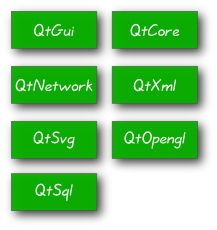
\includegraphics[scale=0.5]{./imagenes/pyqt}
			\caption{Modulos de PyQt}\label{pyqt_modulos}
		\end{figure}	

\newpage			
\newpage
\section{Desarrollo}
  \subsection{Análisis de requerimientos de usuario}
		
			Automatizar la tarea de registro de entrada y registro de salida del laboratorio de computo del Instituto Tecnológico de San Juan del R\'io, es algo que hasta
		d\'ia de hoy se hace de manera manual, anotando en formatos físicos \textit{papel}, la hora de entrada del mismo, en general son los prestadores de servicio social 
		los que se encargan de realizar dicha actividad, que ademas de ser repetitiva y con doble carga de trabajo, pues una vez realizado el registro este, a un tiempo
		determinado tiene  que ser contabilizado y transferido a una base de datos de forma manual.
		
		Como se puede apreciar es un proceso repetitivo y bien definido, que no obstante es propenso a errores humanos o en su defecto a la corrupción del medio físico en 
		el cual se realiza el registro de la información, que ademas es muy limitada en tanto a los datos que provee.
		
		Por esa y algunas otras razones que posiblemente se nos escapen ahora, es que la construcción de un sistema que automatice el proceso y que ademas agregue otras
		funciones deseables, se ve no solo como algo que debe ser implementado sino como una evolución natural del sistema anterior.
		
		Para lograr implementar de forma exitosa el proyecto es necesario que el se cubran los requerimientos funcionales y no funcionales que a continuación se detallan,
		una vez que todos y cada uno de ellos se haya cumplido e integrado en un sistema funcional que cumpla con las especificaciones propuestas, se podrá decir que el 
		sistema esta listo para su uso.
		 	
  \subsection[Requerimientos funcionales]{An\'alisis Requerimientos t\'ecnicos funcionales \label{funcionales}}
		
			Recolectar información es uno de los objetivos primarios, para ello es necesario que el sistema permita realizar ciertas tareas especificas y bien definidas,
		y por medio de ellas obtener el resultado esperado.
		Cada una de la cuales representara un modulo individual, y como la metodología de desarrollo que se utiliza \ref{XP} se fundamenta en el desarrollo de prototipos,
		y iteraciones por cada uno de estos, sera esta pues, la forma en que se trabajara.
		
		Comenzaremos describiendo cada uno de los módulos y su función, iniciaremos por los que están mas cercanos al usuario final, que en este caso son los alumnos y el 
		personal que administre el sistema.
		
		\subsubsection{Interfaz de usuario \label{GUI}}
		
			Una interfaz gráfica de usuario \textbf{GUI} \textit{(por sus siglas en ingles)} que permita la interacción directa con el sistema, 
			clara y fácil de usar.
			Su principal objetivo es que permita al usuario ingresar los datos necesarios para que los diferentes módulos trabajen, del lado de los alumnos la única 
			información requerida es su numero de control y el numero de maquina que ha de usar, ordenar que se genere el registro y listo.
			El resto del trabajo se hace debajo dela capa de abstracción que representa dicha interfaz.
			
			En la misma aparte de los campos para numero de control y maquina, también se deberá desplegar un mapa o diagrama de la distribución de los equipos, en donde 
			de pueda ver los equipos disponibles y los que estén en ocupados en determinado momento.
			
			Todo esto sin olvidar la estética, usabilidad y confiabilidad con la que debe de contar para superar las pruebas de calidad.

		\subsubsection{Interfaces de adminsitraci\'on \label{administracio}}
			
			Ya que se han construido la interfaz para el usuario, se deberá crear un panel de administración, misma que permita configurar ciertos parámetros, realizar
			consultas y motitorear el funcionamiento del sistema en general.
			
			En esta primera version funcional dicha interfaz no contara con todos los controles disponibles, gradualmente conforme se avance en el desarrollo del proyecto
			se irán agregando funcionalidades cada que estén listas y se acoplen perfectamente con el resto del sistema, de acuerdo al funcionamiento de la metodología que
			se ha implementado en el desarrollo.
		
		\subsubsection{Validar \label{validar}} 
			Las interfaces de usuario y de administración alimentan al sistema para que funcione, sin embargo la información que se introduce debe de ser valida, y cumplir 
			con ciertos requisitos, de lo contrario al intentar procesar los datos estos  que el sistema se salga de los  establecidos y por lo tanto 
			cause que el mismo falle y en el peor de los casos termine su ejecución con la posible perdida de información.
			
			Para evitar este tipo de fallo es necesario implementar mecanismos que permitan validar que la información que se introduce es la correcta, básicamente son solo
			dos los valores que se introducen por parte del usuario, su numero de control y el n\'umero de m\'aquina que usara, por lo que los podemos integrar la validación
			de ambos en un solo modulo que se encargue de analizar y retornar una respuesta al programa principal.
			
			Validar el n\'umero de control del alumno consta de los siguientes puntos, mismos que se deben cumplir para que la misma sea exitosa:
			\begin{itemize}
				\item Sintaxis
				\item Existencia \footnote{\scriptsize \textit{Se refiere al echo de si el alumno esta activo o dado de baja en el sistema \gls{SII}.}}
			\end{itemize}
			Como se puede ver, son solo dos puntos, mismo que se eben cumplir sin excepción alguna, pues de lo contrario no puede continuar el proceso de registro.
		\subsubsection{Obtener datos relacionados \label{relacionados}}
			Cuando se valida en numero de control, y ser determina que si sintaxis cumple con las ciertas características, lo siguiente es extraer los datos que estén 
			asociados a ese numero de control, mismo que internamente se maneja como la clave principal de cada uno de los alumnos, a si mismo todos y cada uno de los datos
			almacenados esta intrínsecamente ligado a una clave.
			Los datos que se recolectan son los siguientes:
			\begin{itemize}
				\item N\'umero de control
				\item Nombre
				\item Apellido Paterno
				\item Apellido Materno
				\item Carrera (\textit{Especialidad})
			\end{itemize}
			
			Por lo que cuando el alumno ingrese su numero de control, el sistema después de validarlo, realiza una consulta a la base de datos, esto con la finalidad en un
			principio, de determinar que en efecto existe en la misma.
			Posteriormente si existe, retorna los datos del alumno, mismo que se mostraran en campos especialmente reservados para tal fin el formulario de registro \ref{GUI}.
			
			Dichas tareas se realizaran de forma transparente al usuario, que apenas detectara que se tarda en efectuarlas.
		\subsubsection{Numero de m\'aquina \label{maquina}}
			
			Ya se vio  que se espera de la validación de los datos que se introducen por parte del usuario en la  \ref{validar} se describe.
			Una vez que se verifica que el alumno exista en la base de datos, se visualizan los datos del mismo en el formulario de registro, de procede a validar la m\'aquina
			que quieres usar, en este punto se debe comprobar lo siguiente:
			\begin{itemize}
				\item Sintaxis
				\item Disponibilidad  \footnote{\scriptsize \textit{Si esta libre u ocupada, según corresponda}}
				\item Existencia \footnote{\scriptsize \textit{No confundir con el estatus de alumnos, en esta caso indica si esta funcional o no la maquina.}}
			\end{itemize}
			Si los puntos anteriores se satisfacen con éxito, el proceso continua.
			
		\subsubsection{Preparar registro \label{consulta}}
			Una vez que todos los datos han sido validados y recolectados se procede a preparar la consulta, o en otros términos recolectar los datos necesarios para efectuar
			el registro de entrada o de salida en la base de datos, que si todo el proceso ha sido exitoso no conlleva ninguna complejidad.
			Los datos en cuestión son los siguientes:
			\begin{description}
				\item[ID]: un identificador auto-generado y con incremento automático, para identificar el registro. 
				\item[N\'umero de control]: puede ser el que introduce el usuario o el que se lee de la base de datos.
				\item[N\'umero de m\'aquina]: la maquina que usara.
				\item[Fecha de entrada]: en formato \texttt{AAAA-MM-DD}.
				\item[Hora de entrada]: en formato \texttt{H:M:S}.
			\end{description}
			La fecha y hora se obtienen directamente de los que maneja el sistema, una función especial se encarga de obtener dichos datos.
		
		\subsubsection{Restablecer el formulario}
		
			Una vez que se ha realizado con \'exito el registro de entrada \'o salida, se procede a limpiar el contenido de los campos del formulario, y eliminar el contenido de 
			las variables usadas internamente, dejando listo el sistema para un nuevo registro.
			El sistema entonces entra en estado de espera, hasta que detecta que el campo correspondiente al numero de control ha cambiado, pasando de estar vació a contener 
			alguna cadena de caracteres, entonces comienza el ciclo nuevamente.

		\subsubsection{Ampliaciones a futuro}
			Los módulos contenidos hasta este punto, as\'i como su función son los mínimos y estrictamente requeridos para que el sistema funcione de manera básica, 
			posteriormente en futuras iteraciones la funcionalidad del mismo se extenderá considerablemente, obviamente por cada una de ellas que sea integrada se agregara su
			respectiva sección en este documento. 


		
  \subsection[Requerimientos no Funcionales]{An\'alisis de requerimientos t\'ecnicos no funcionales}
  		En esta sección se describen los elementos que si bien no son componentes clave del sistema, son necesarios para que el mismo funcione de forma adecuada, en el estado
  		actual de desarrollo esto son m\'as bien pocos.
  		
		\subsubsection{Disponibilidad}
			El periodo de operación debe ser de trece horas cada día hábil de la semana, lo que generalmente es de lunes a viernes de \textsc{07:00} a \textsc{20:00}, lapso 
			en el cual debe estar en pleno funcionamiento y disponibilidad.
			
			Dado que el sistema se instalara en una maquina dedicada únicamente para este fin, dicho equipo deberá ser configurado para solo funcionar para determinas tareas
			que serán descritas en puntos posteriores.
			
		\subsubsection{Accesibilidad}
			Las interfaces de usuario se han pensado para ser fáciles de usar, y con apenas interacción con el usuario, fuera de las tres pasos que debe realizar para proveer 
			los datos necesarios al sistema:
			\begin{enumerate}
				\item Ingresar n\'umero de control.
				\item Seleccionar una m\'aquina.
				\item Pulsar la tecla \texttt{Enter} para efectuar el registro.
			\end{enumerate}
			Como se puede ver el nivel de interacción por parte del usuario es muy simple, el dise\~no de la interfaz es también simple y visualmente confortables.
			En la figura \ref{user_gui} se puede ver el aspecto de la interfaz de usuario.
			\begin{figure}[h!]%Ambiente ’figure’
				\centering
				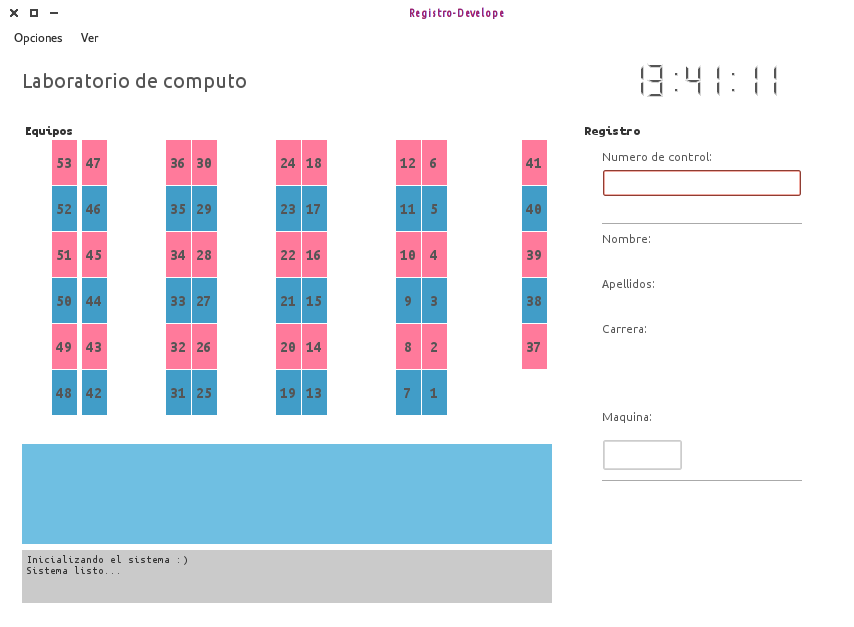
\includegraphics[scale=0.5]{./imagenes/user_gui}
				\caption{Interfaz de usuario.}\label{user_gui}
			\end{figure}
			En donde se puede comprobara que es accesible.

		\subsubsection{Rendimiento}
			La elección de las plataformas de desarrollo fueron especialmente pensadas para este proyecto, por un lado el lenguaje de programación  \texttt{Python} \ref{python}
			es ideal para sistemas modulares que requieran de un desarrollo acelerado, pese a ser un lenguaje interpretado es lo bastante rápido para ser usado en proyectos
			importantes, no por nada es usado por grandes empresas como \textsf{Google}.
			Por el lado de las librerías gráficas, \texttt{QT}, aunque mas específicamente \texttt{PyQt} \ref{pyqt}, que es el port la primera para ser usada con Python, es
			multi-plataforma y una de las librerías gráficas mas poderosas.
			
			Por ultimo todo esto se instalara en sistema operativo de tipo \texttt{UNIX}, mas específicamente una distribución linux, \texttt{Manjaro}, misma que se selecciono
			por algunas razones, entre ellas esta la fácil configuración del sistema, la facilidad de uso para los usuarios que no estan acostumbrados a entornos 
			\texttt{GNU/Linux}.
			
			En resumen se puede estar seguro que con la elección de tecnologías mencionadas hasta este punto, el sistema rendirá como se espera y cumplirá sin problema alguno 
			con los requisitos de funcionales previamente documentados \ref{funcionales}
		
		\subsubsection{Escalabilidad, mantenibilidad y portabilidad}
			Las herramientas y sistema operativo seleccionado, fueron pensadas para proporcionar desde un principio todas estas posibilidades, desde el side\~no mismo del
			sistema, hasta las posibles arquitecturas en las cuales se implemente.
			
			Por el momento solo hay una restricción, no se puede ejecutar en dispositivos móviles.
			
  \subsection{Dise\~no \label{dise}}
  		Una vez identificados los requerimientos funcionales y no funcionales del sistema, crear un modelo de como debería ser cada uno de los componentes del sistema es posible
  		pero m\'as que posible es algo que se debe hacer a vistas de continuar con la siguiente etapa del proceso, desarrollo, implementaci\'on y pruebas.
  	
	  	\subsubsection{Dise\~no del núcleo de la aplicación}
			El n\'ucleo del sistema es relativamente simple, consta de los siguientes pasos:
			\begin{enumerate}
				\item Introducir numero de control.
				\item Validar numero de control.
				\item Obtener datos relacionados a dicho n\'umero de control.
				\item Seleccionar equipo.
				\item Recolectar y preparar la consulta de registro.
				\item Realizar registro.
				\item Inhabilitar el equipo seleccionado.
				\item Restablecer los formularios.
			\end{enumerate}
			Esto para el proceso de registro de entrada, aunque el proceso es exactamente el mismo para registrar la salida del mismo, salvo por que en vez de inhabilitar se 
			libera el equipo en cuestión, que vuelve a estar disponible para futuros usuarios.
			
			El diagrama de flujo de la figura \ref{user_flow} ilustra el proceso de registro de un usuario.
			\begin{figure}[h!]%Ambiente ’figure’
				\centering
				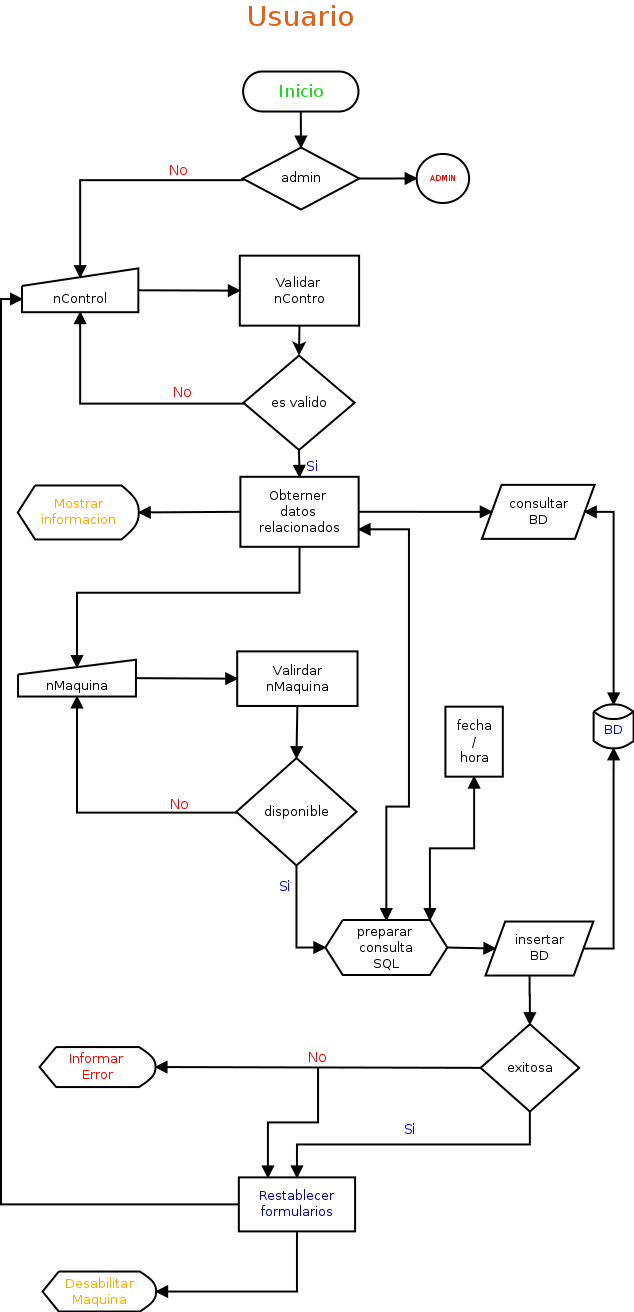
\includegraphics[scale=0.4]{./imagenes/flujo_usuario}
				\caption{Proceso de registro.}\label{user_flow}
			\end{figure}			
		
		\subsubsection[GUI]{Dise\~no de la interfaz de usuario}
			La interfaz de usuario es la misma que se muestra en la figura \ref{user_gui}, ahora solo describiremos sus elementos:
			\begin{enumerate}
				\item N\'umero de control para introducir el n\'umero de control.
				\item Datos de alumno cuando se valida que el n\'umero de control es valido, se llenan automáticamente con los datos de este.
				\item N\'umero de m\'aquina el equipo que se usara.
				\item Diagrama del laboratorio muestra la distribución de los equipos en el laboratorio de computo. 
				\item Estadísticas diarios muestran cierta información sobre el uso del laboratorio a lo largo del día.
				\item Log del sistema muestra información relacionada a la operación que se realiza en el momento.
			\end{enumerate}
			La imagen de la figura muestra los puntos arriba mencionados.
			\begin{figure}[h!]%Ambiente ’figure’
				\centering
				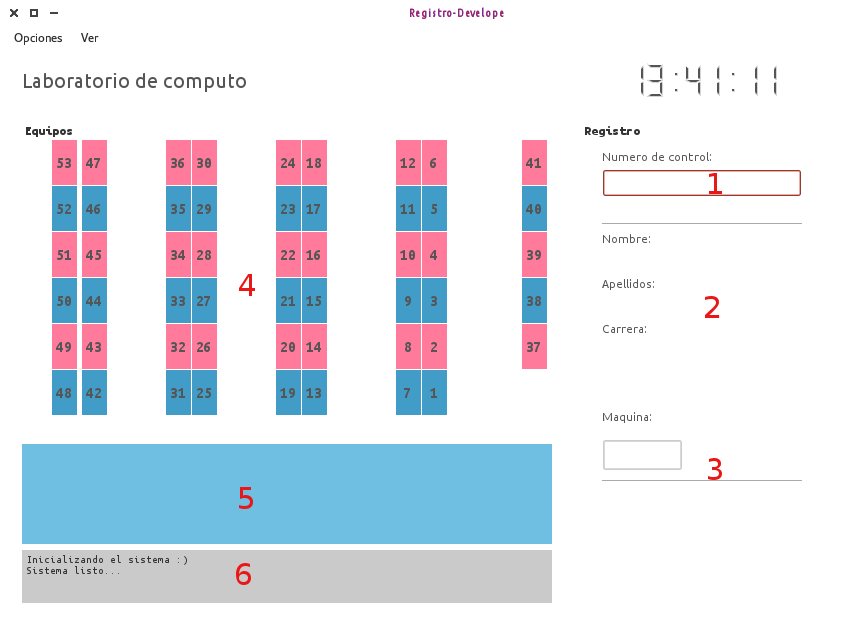
\includegraphics[scale=0.4]{./imagenes/user_gui_num}
				\caption{Secciones de la interfaz de usuario.}\label{user_gui_num}
			\end{figure}
		
		\subsubsection[Base de datos]{Dise\~no de la base de datos}
			De la mano del núcleo del sistema, fue necesario dise\~nar una base de datos que permitiera almacenar los datos que se generan, es simple, pero sin ella no seria
			posible que el sistema cumpla con los objetivos planteados, hasta el momento se compone de tres tablas:
			\begin{description}
				\item[Alumnos] almacena los datos de los alumnos activos en el SII.
				\item[Entrada] almacena los datos de entrada.
				\item[Salida] para cada entrada ingresa una fecha y hora de salida.
			\end{description}

  \newpage  
  \subsection{Implementaci\'on}
		
	\subsubsection[Base de datos]{Construcci\'on de la base de datos}
		La base de datos es la parte central de todo el sistema, pues es donde se almacenaran los datos generados por el sistema, para los fines que después se requieran
		por ello y seleccionar un manejador de base de datos compatible con las tecnologías usadas es de gran importancia, la opción fue usar \texttt{MariaDB}, la cual es
		en términos simples una version de \texttt{MySQL} potenciada y con muchas características a\~nadias que lo hacen ideal para ser el motor de base de datos.
		
		En la imagen \ref{db_reg} podemos ver la estructura de las tablas que componen la base de datos.
		\begin{figure}[h!]%Ambiente ’figure’
			\centering
			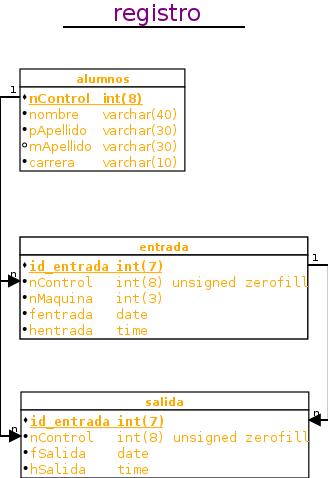
\includegraphics[scale=0.5]{./imagenes/db_registro}
			\caption{Tablas de la base de datos}\label{db_reg}
		\end{figure}
	\subsubsection[Modulos]{Construcci\'on de los m\'odulos de sistema}
		La metodología elegida exige la cosntruccion de prototipos, lo que es lo mismo, cada uno de los modulos descritos la seccion \ref{funcionales} se construyo por separado,
		con los elementos estrictamente necesarios para su funcionamiento.
		
		Siendo agregados al proyecto solo y únicamente hasta que estuvieron completos y funcionales.
		
		Explicar el funcionamiento interno de cada modulo, escapa de las posibilidades de este documento, mas no significa que la documentación no exista, esta est\'a alojada
		en el sistema de control de versiones \texttt{CVS}, \texttt{GitHub}, en el siguiente enlace, el repositorio por el momento esta administrado por 
		\textsf{Juan Carlos \'Avila}, aunque se puede ramificar por quien guste.
		
		\href{http://github.com/karlislee/sistema-de-control}{Sistema para el registro de entradas y salidas de áreas criticas \textsl{GitHub}}
		el documento esta perfectamente documentado, en cada una de las funciones y clases que lo componen, por lo que incluir la descripción lógica de los mismos seria 
		redundante, para ello revise la documentación de cada modulo en el repositorio.
		
	\subsubsection{Problemas por resolver}
		En este punto y pese a que el sistema es funcional, aun hay detalles que arreglar, en especial del lado del administrador del mismo, de nuevo cada uno de los elementos
		que se agreguen, serán debidamente documentados tanto en este documento como en el correspondiente a cada nuevo modulo generado, todo esto alojado en el repositorio 
		del proyecto.
	
  \subsection{Pruebas}
		Las pruebas que se aplicaron al sistema se basan en las pruebas fueron las que recomienda la metodología usada \ref{XP}, son las pruebas unitarias, las cuales son en
		resumen pruebas aplicadas durante el proceso iterativo del desarrollo, la idea general es desarrollar un módulo o función por separado o con los mínimos
		elementos para que funcione y una vez que se superan las expectativas esta se integra en el sistema principal en donde se hace la segunda prueba o de integración.

		En este caso cada una de las funciones que lo permitían se crearon por separado, y una ves que estuvieron funcionando se integraron con el resto del sistema, de esta
		forma solo las piezas que en efecto cumplían con su objetivo, se agregaron al conjunto de funciones o definiciones que componen el resto del sistema.
		
		Cada que una nueva funcionalidad se agrego al proyecto, este se guardo como una instantánea del sistema, esto para que los cambios futuros se agreguen a una versión 
		actualizada del mismo.
		\subsubsection{Resultados de las pruebas}
			Dada la metodología los resultados de las pruebas ya sean buenas o malas se corrigen en el momento, pues si la nueva funcionalidad que se este construyendo, no supera
			satisfactoriamente las mismas, esta no puede ser agregada al sistema.
			En pocas palabras una función no esta lista hasta que no este lista.
		
		\subsubsection{Mejoras realizadas después de las pruebas.}
			Dada la naturaleza de metodología y como ya se menciono anteriormente, las pruebas se implementan en el mismo proceso de desarrollo, con las pruebas unitarias, lo que
			hace que cuando una nueva función se agrega al sistema, esta ya esta ya a superado las pruebas necesarias, por lo que las pruebas del sistema en general no llegan a
			darse.
			
		\subsubsection{Detalles pendientes por arreglar}
			
  \subsection{Resultados obtenidos}
  	En este punto de la iteraci\'on el sistema esta en una etapa funcional, al menos en lo que se refiere al funcionamiento general, funciona en lo que corresponde al enviar
  	y recibir mensajes, la conexión al sistema y proceso de validación funcionan, a\'un no se ha implementado una forma de mantener los datos en una base de datos no obstante
  	para el siguiente prototipo sera una de las principales funciones a implementar, justo con un formulario  de registro.
  	
  	El aplicar los pasos de la metodología de desarrollo extremo, brinda resultados en poco tiempo de desarrollo, mientras que si las características cumplen o no con las 
  	funcionalidades esperadas, estas se pueden cambiar o mantener para próximas generaciones generando a\'un as\'i prototipos funcionales en cada iteraci\'on.
	
  \subsection{Conclusión}
  
  	Realizar este proyecto ha sido de gran ayuda, tanto profesional como personal, pues cada vez profundizo mas en esas actividades que tanto me apasionan, conocer mas
  	características y posibilidades de los lenguajes y librerías que se usaron para el desarrollo del sistema.
  	Es solo el comienzo, mejores cosas están por venir creo que lo ideal seria construir un sistema genérico que pueda adaptarse a cualquier problemática de registro de 
  	entradas y salidas.
  	Si bien es posible que ya existan sistemas de este tipo, para mi la motivaci\'on es m\'as que nada por el carácter didáctico, pues a fin de cuentas estoy en proceso de 
  	preparación.
  	Si hay algo que aprendí, es que la disciplina puede hacer las cosas mas fáciles, creo que sera algo que ponga en practica en mis proyectos futuros y en las mejoras que 
  	tengo contempladas para este mismo.
%----------------------------------------------------------------------------------------
%	BEGIN GLOSARIO
%----------------------------------------------------------------------------------------			
\newpage


\printnoidxglossaries
\pagenumbering{roman}
%----------------------------------------------------------------------------------------
%	END GLOSARIO
%----------------------------------------------------------------------------------------

\newpage

%---------------------------------------------------------------------------------------
%	BIBLIOGRAPHY
%----------------------------------------------------------------------------------------

\begin{thebibliography}{99} % Bibliography - this is intentionally simple in this template




\bibitem{Luckham} 
David Luckham
[\textit{The Power of Events - An Introduction to Complex Event Processing in Distributed Enterprise Systems}]. 
Addison-Wesley, ISBN 0-201-72789-7.


\bibitem{Tello} 
Adolfo Lozano Tello
[\textit{Iniciación a la programación utilizando lenguajes visuales orientados a eventos.}] [ISBN978-84-7897-714-7]
Ed.Bellisco Ediciones Técnicas y Científicas, ISBN 84-95279-49-5. ISBN 978-84-95279-49-1.


%\bibitem{} 
%Ricardo Barona Vázquez
%[\textit{Asterisk©, telefonía IP en software libre}].
%\href{Asterisk}{ http://www.enterate.unam.mx/artic/2008/abril/art3.html}

\end{thebibliography}


%----------------------------------------------------------------------------------------
 
\end{document}

